\documentclass[12pt,a4paper]{article}
\usepackage[utf8]{inputenc}
\DeclareUnicodeCharacter{00A0}{ } 

\usepackage[T1]{fontenc}
\usepackage{lmodern}
\usepackage{geometry}
\usepackage{hyperref}
\usepackage{booktabs}
\usepackage{parskip}
\usepackage{titlesec}
\usepackage{xcolor}
\usepackage{listings}
\usepackage{graphicx}
\usepackage{float}

\lstset{
  basicstyle=\ttfamily\small,
  frame=single,
  backgroundcolor=\color{gray!10},
  breaklines=true,
  numbers=left,
  numberstyle=\tiny\color{gray},
  keywordstyle=\color{blue}\bfseries,
  stringstyle=\color{red}
}

\geometry{margin=2.5cm}

\hypersetup{
    colorlinks=true,
    linkcolor=blue!60!black,
    urlcolor=blue!60!black,
}

% IL PROBLEMA ERA QUI: \titrule è stato corretto in \titlerule
\titleformat{\section}{\large\bfseries}{}{0em}{}[\titlerule]
\titleformat{\subsection}{\normalsize\bfseries\itshape}{}{0em}{}

\title{\textbf{Relazione Finale Completa}\\[0.4em]
       \large Progetto: Agenti RL e Integrazione LLM/VLM in MiniGrid-DoorKey}
\author{}
\date{\today}

\begin{document}

\maketitle
\tableofcontents
\bigskip

\section{Panoramica del Progetto}
Il progetto analizza l'efficacia di diversi paradigmi di apprendimento per rinforzo (RL) e l'integrazione di modelli di visione e linguaggio (VLM/LLM) nell'ambiente \texttt{MiniGrid-DoorKey} di Gymnasium. Il compito dell'agente è sequenziale: localizzare una chiave, raccoglierla, aprire una porta chiusa e raggiungere l'obiettivo finale (casella verde). La sfida principale risiede nella natura sparsa del reward originale, affrontata in questo lavoro tramite un sistema di \textit{Reward Shaping} denso e l'ausilio di modelli linguistici per la valutazione delle azioni.

\section{Configurazione dell'Ambiente e Reward Shaping}
Per superare i limiti del reward ambientale, è stato implementato il modulo \texttt{env/rewardsystem.py} che introduce un segnale denso basato sugli stati logici del task (\texttt{Stage}).

\subsection{Componenti del Reward}
Il reward totale è calcolato come somma di componenti configurabili tramite \texttt{RewardConfig}:
\begin{itemize}
    \item \textbf{Potential-based shaping}: implementato secondo la formula $F(s,s') = \gamma\,\Phi(s') - \Phi(s)$, dove $\Phi$ rappresenta il progresso BFS verso l'obiettivo corrente (chiave, porta o goal). Gli iperparametri scelti sono \textit{Shaping Scale} a $0.7$ e \textit{Gamma} ($\gamma$) a $0.995$.
    \item \textbf{Bonus Milestone}: premi una-tantum per il completamento delle fasi ($+0.5$ per chiave/porta, $+1.0$ per il goal).
    \item \textbf{Penalità}: una penalità temporale costante per step e una penalità di regressione per il ritorno a fasi precedenti.
\end{itemize}

\section{Architetture degli Agenti}
\subsection{Q-Learning Tabellare (\texttt{agent/doorkey-reward-machines-wandb.py})}
L'agente classico utilizza uno stato compresso $(\Delta x, \Delta y, d, \text{progress}, \text{stage})$ il quale fornisce all'agente osservazioni sulla sua posizione relativa al goal corrente, la sua direzione, il progresso (arrotondato secondo un dato numero di bin), e il numero di stage corrente.


\subsection{Double DQN con PER (\texttt{agent/doorkey-DDQN.py})}
L'agente Deep RL utilizza una rete \texttt{DualHeadDDQN} che elabora separatamente l'immagine della griglia (tramite \textit{Grid MLP}) e feature scalari quali direzione e progresso. La motivazione dietro a questo approccio era di dare valore alle feature scalari provenienti da \textit{rewardsystem.py} che se aggiunte all'immagine dell'ambiente si sarebbero a mio avviso perse nei "pixel" dell'immagine linearizzata.


\newpage
\section{Sperimentazione LLM e VLM}
L'integrazione del \texttt{VLMDebugWrapper} permette di iniettare nel loop di RL un reward derivato dall'analisi dei frame o dello stato testuale.

\subsection{Ingegnerizzazione del Prompt}
Per forzare il modello a ragionare in modo analitico, è stato sviluppato un prompt strutturato che richiede un'analisi in 5 step (Target, Azione precedente, Analisi Spaziale, Stima del progresso, Calcolo del reward).

\begin{quote}
Il prompt descrive un sistema di valutazione per un agente intelligente operante in un ambiente \textit{GridWorld} 2D sconosciuto. L'agente dispone di un insieme limitato di azioni (rotazione sinistra/destra, avanzamento, raccolta, deposito e interazione con oggetti) e deve raggiungere un obiettivo finale rappresentato da una cella verde, superando eventuali ostacoli come porte chiuse che richiedono chiavi corrispondenti. Il sistema istruisce un modello linguistico ad agire come ``occhio e cervello'' dell'agente, seguendo una sequenza rigorosa di cinque passi analitici: identificazione del target corrente, valutazione dell'azione precedente, analisi spaziale e di orientamento, calcolo di una ricompensa numerica compresa nell'intervallo $[-1.0, 1.0]$ secondo criteri gerarchici predefiniti (da azione stupida a obiettivo finale raggiunto), e stima del progresso globale dell'agente nell'intervallo $[0.0, 100.0]$. Il risultato atteso è un output in formato XML strutturato, contenente il ragionamento nell'elemento \texttt{<analysis>} e le due metriche numeriche nell'elemento \texttt{<metrics>}, senza alcun testo aggiuntivo al di fuori di tali tag.
\end{quote}

\paragraph{Prompt leggibile nel file:}
\begin{quote}
    \texttt{/src/internship/env/vlm\_wrapper.py}
\end{quote}


\subsection{Prove LLM}
Nelle prove puramente testuali, la griglia viene convertita in formato CSV. I modelli (Gpt-oss-120b, Qwen3.6-36b) hanno dimostrato di comprendere la gerarchia degli obiettivi (chiave prima della porta), ma faticano a percepire correttamente la direzione in cui l'agente è rivolto senza un feedback visivo diretto.

Il Prompt in questo caso è stato una versione molto simile a quello utilizzato con i modelli LLM modificato per far comprendere le immagini input.

\subsection{Prove VLM: Il benchmark Qwen-27B}
L'uso di modelli multimodali ha risolto le ambiguità spaziali. 
\begin{itemize}
    \item \textbf{Modelli Small (4B-14B)}: (es. \texttt{nemotron-3-nano}, \texttt{Qwen-vl-4b}) mostrano spesso allucinazioni sulla posizione degli oggetti o sull'orientamento.
    \item \textbf{Qwen-27B}: Questo modello ha rappresentato il punto di svolta. È stato in grado di fornire risultati \textbf{decisamente soddisfacenti e coerenti}, identificando con precisione la relazione tra l'agente e il target, garantendo una valutazione del reward abbastanza solida, nonostante ogni tanto, a causa forse della risoluzione dell'immagine, sbagliasse a riconoscere il colore della chiave.
\end{itemize}

\section{Risultati e Riepilogo Visivo}
I grafici estratti da Weights \& Biases evidenziano il successo del sistema di reward shaping, confrontando l'allenamento dell'agente con la reward densa e senza (lasciandogli solo le osservazioni).

\begin{figure}[H]
    \centering
    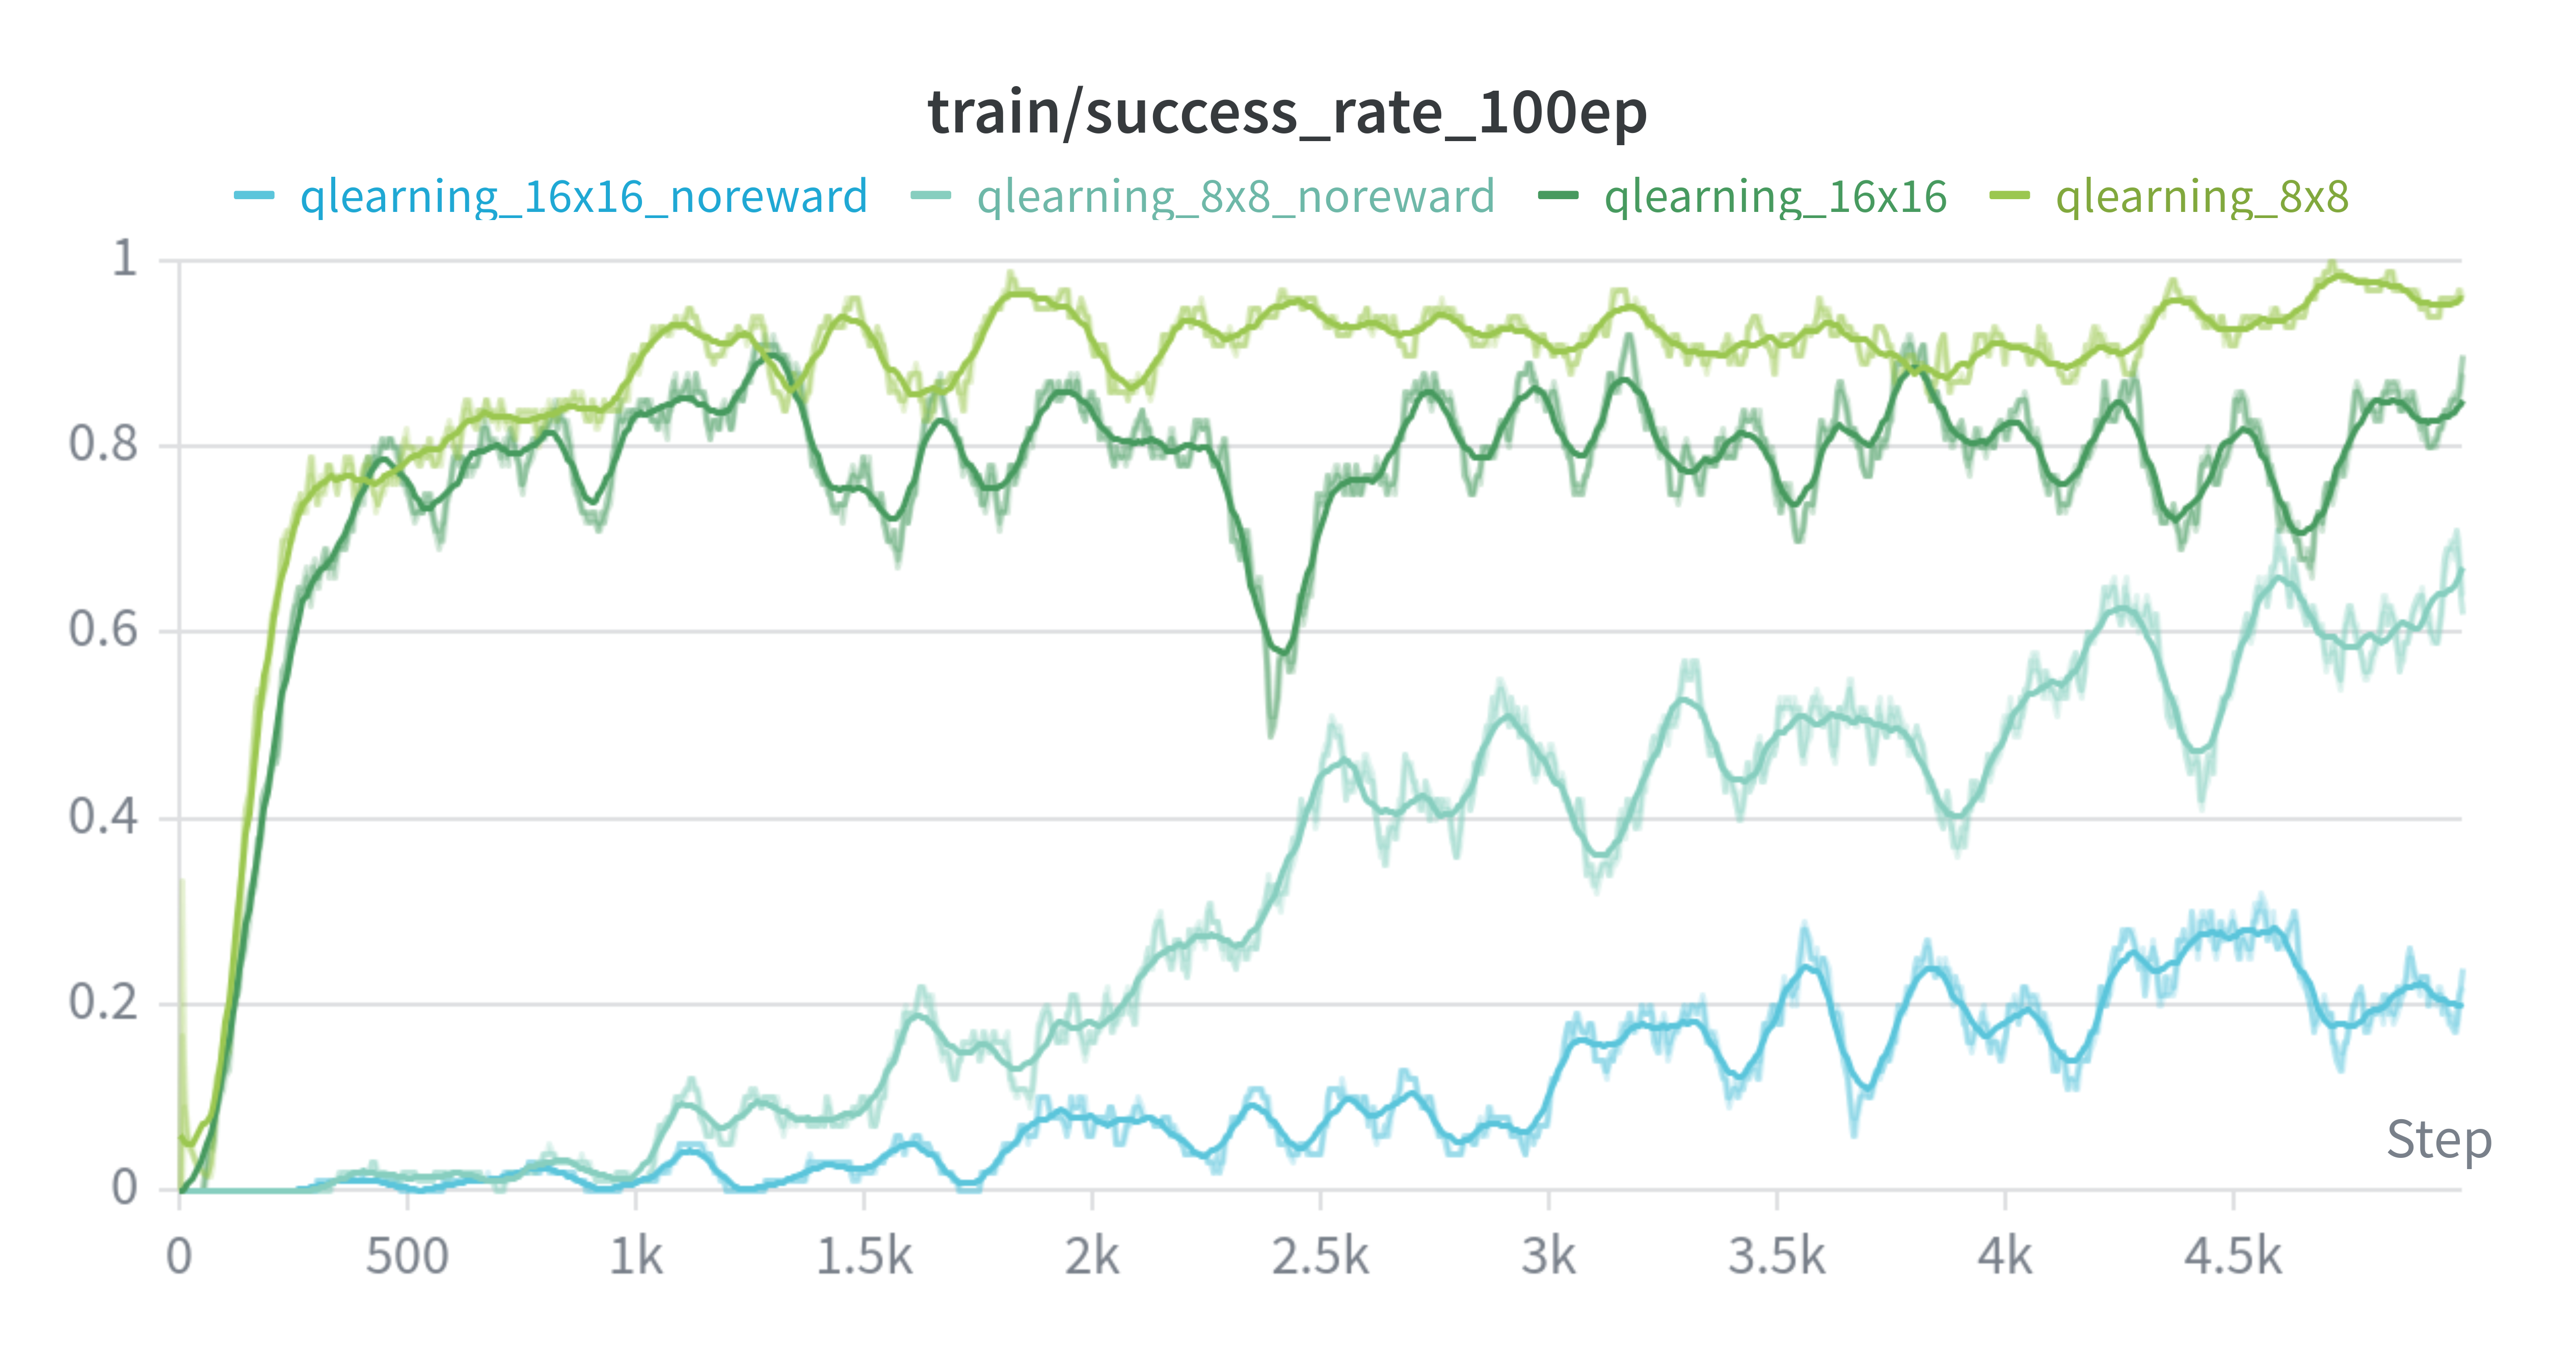
\includegraphics[width=0.85\textwidth]{images/img1.png}
    \caption{Success Rate Q-Learning: Lo shaping permette la risoluzione di mappe $16\times16$ (verde scuro), altrimenti impossibili per la baseline (azzurro).}
\end{figure}

\begin{figure}[H]
    \centering
    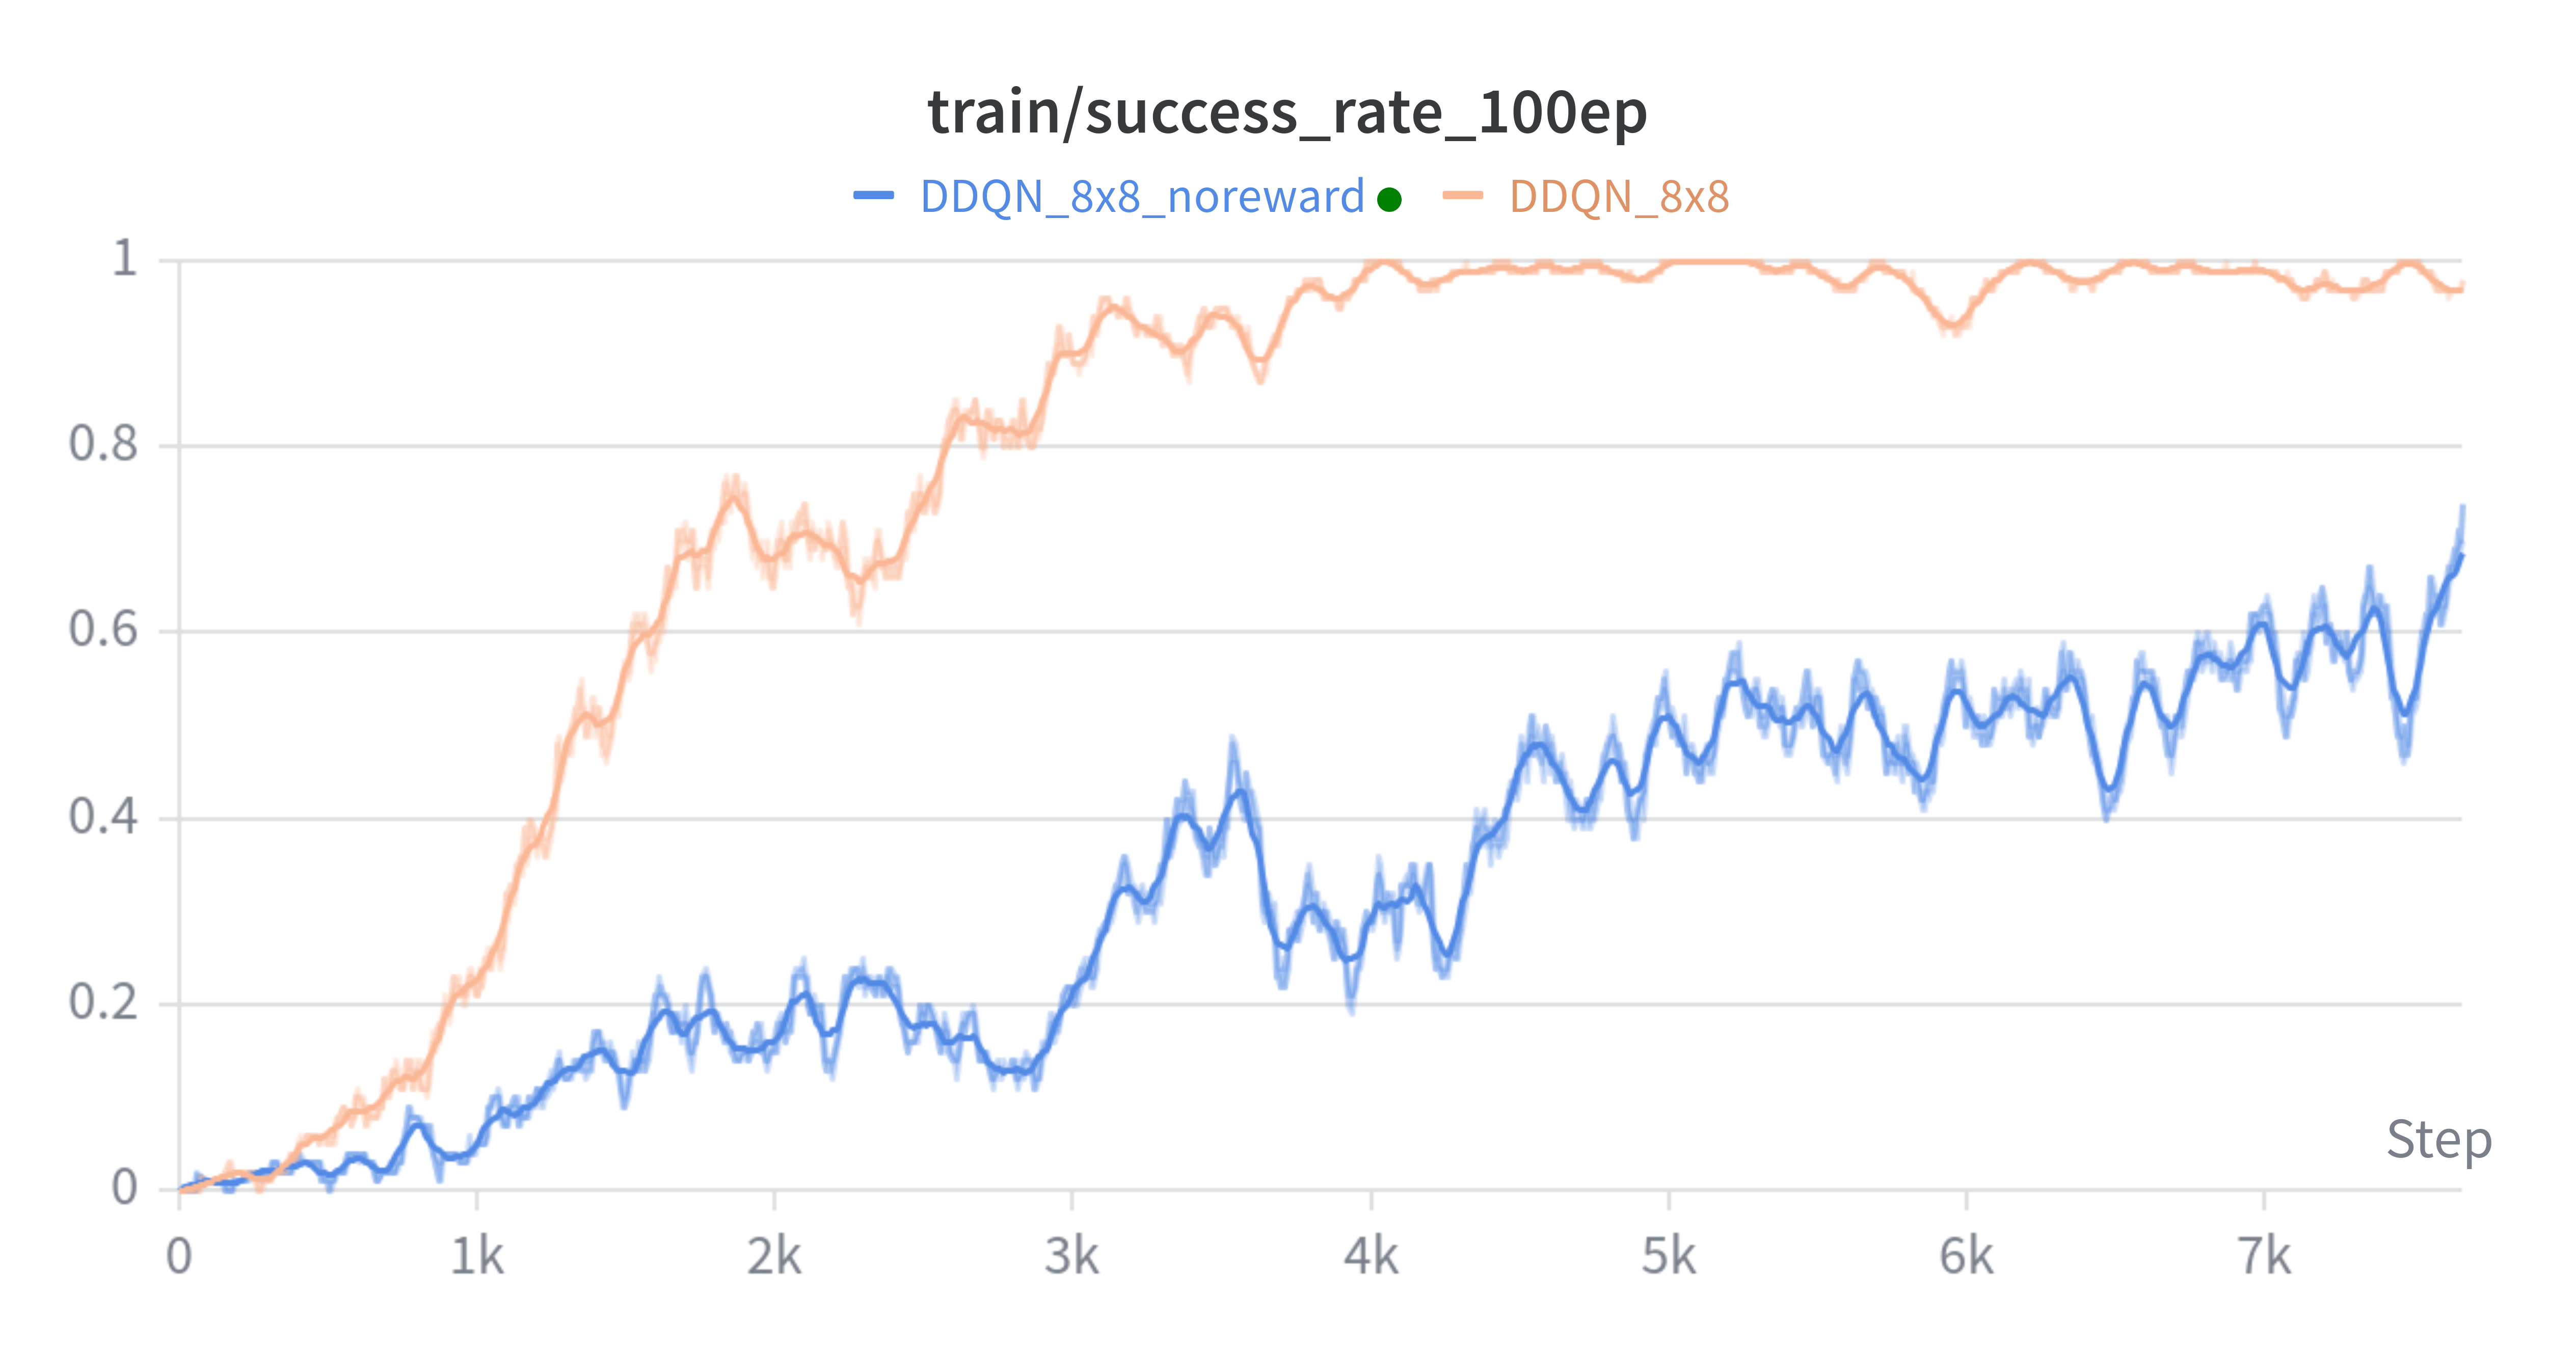
\includegraphics[width=0.85\textwidth]{images/img2.png}
    \caption{Success Rate DDQN 8x8: L'arancione mostra una convergenza rapida al 90\% grazie al reward denso.}
\end{figure}

\begin{figure}[H]
    \centering
    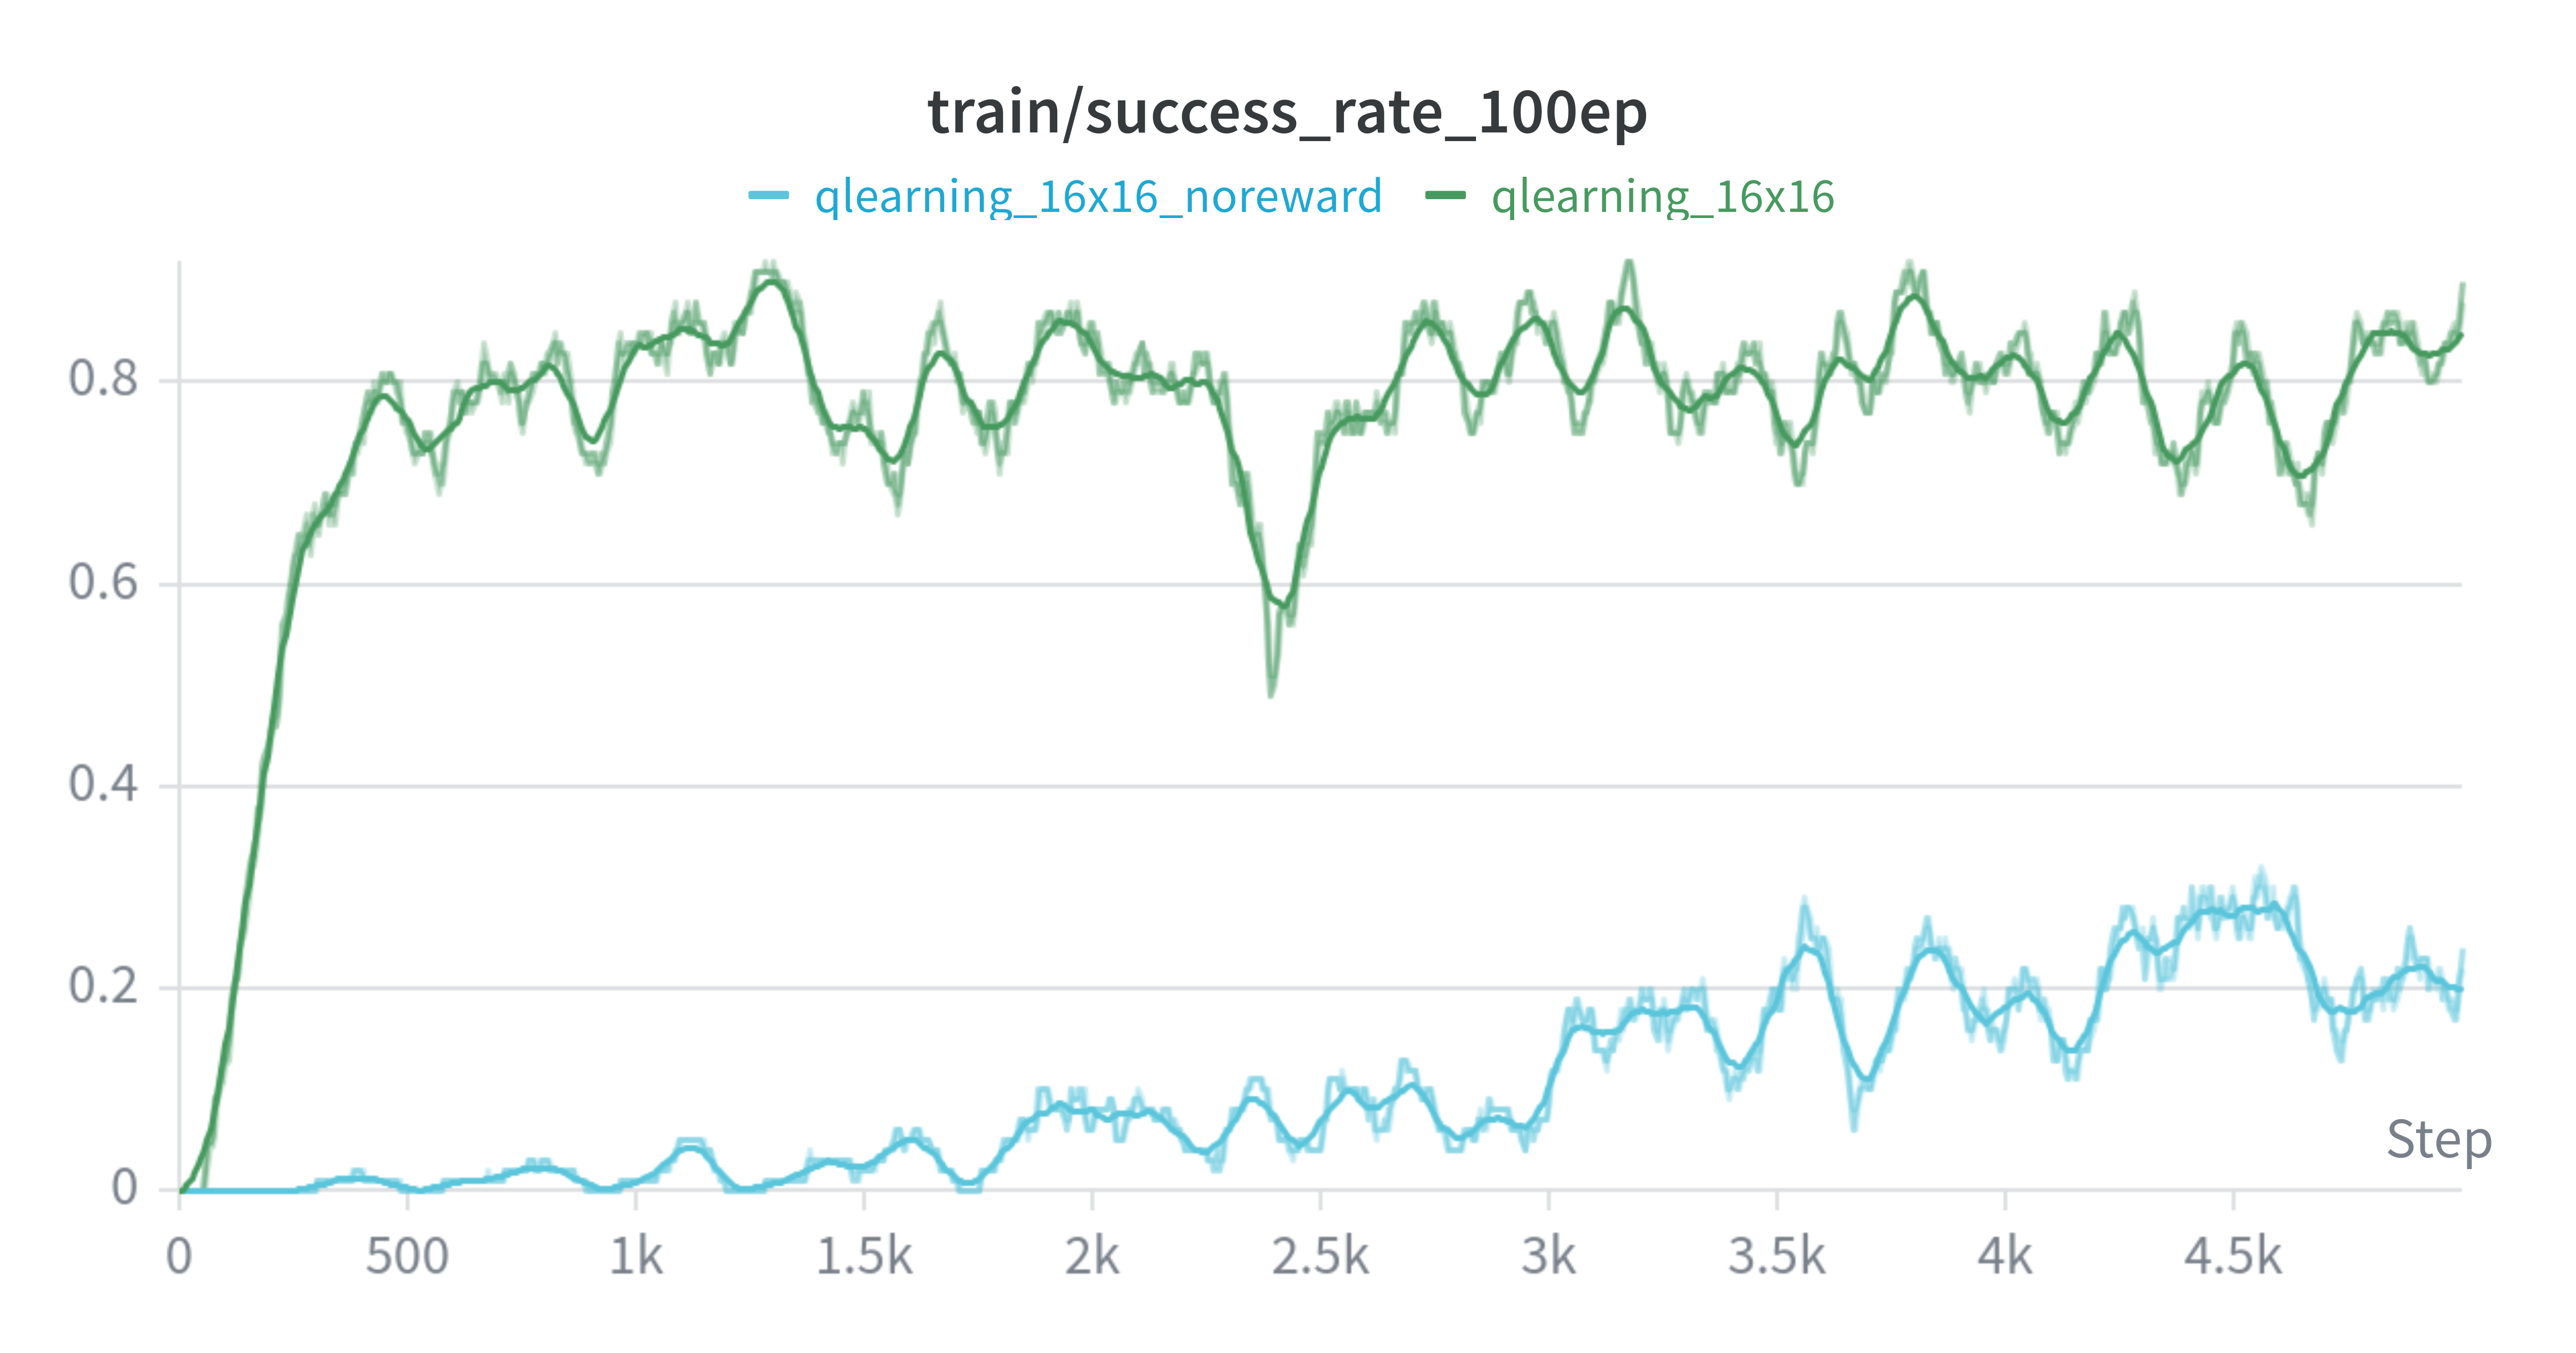
\includegraphics[width=0.85\textwidth]{images/img3.png}
    \caption{Analisi comparativa finale: Dinamiche di convergenza estratte dai log WandB.}
\end{figure}

\subsection{Considerazioni Finali e Sviluppi Futuri}
Nonostante le ottime prestazioni, esistono ampi margini di ottimizzazione nel fine-tuning degli iperparametri (dimensione del buffer e frequenza update). È importante sottolineare che, per questioni legate alle tempistiche computazionali e al tempo complessivo a disposizione, i training non sono stati protratti oltre un certo limite. Tuttavia, l'andamento delle curve suggerisce che \textbf{sessioni di addestramento più lunghe} porterebbero certamente a \textit{success rate} ancora più elevati e stabili, consolidando la policy vicino alla perfezione anche nelle configurazioni più complesse.

\end{document}
